Let 
\begin{align}
\vec{p} = \myvec{4\\3} , \vec{q} = \myvec{– 1\\4}
\end{align}
%
In general, the equation of the ellipse passing through $\vec{p}, \vec{q}$ can be expressed as
\begin{align}
\brak{\vec{x}-\vec{c}}^{\top}\vec{D}\brak{\vec{x}-\vec{c}}=1\label{quadforms/37/eq:14}
\end{align}
where the center $\vec{c}=\myvec{\beta\\0}$ and 
 $\vec{D}$ is a diagonal matrix.
$\because \vec{p}, \vec{q}$ satisfy \eqref{quadforms/37/eq:14},
\begin{align}
\label{quadforms/37/eq:ellipse_std_ab}
(\vec{p}-\vec{c})^{\top}\vec{D}(\vec{p}-\vec{c}) &= 1,
\\
(\vec{q}-\vec{c})^{\top}\vec{D}(\vec{q}-\vec{c}) &= 1,
\end{align}
which can be simplified as 
\begin{align}
    2\brak{\vec{p}-\vec{q}}^{\top}\vec{D}\vec{c}=\vec{p}^{\top}\vec{D}\vec{p}-\vec{q}^{\top}\vec{D}\vec{q}
\end{align}
Using the identity, 
\begin{multline}
    \brak{\vec{p}-\vec{q}}^{\top}\vec{D}(\vec{p}+\vec{q})
   =\vec{p}^{\top}\vec{D}\vec{p}-\vec{q}^{\top}\vec{D}\vec{q}
\end{multline}
in the above, 
\begin{multline}
    2\brak{\vec{p}-\vec{q}}^{\top}\vec{D}\vec{c}  = \brak{\vec{p}-\vec{q}}^{\top}\vec{D}(\vec{p}+\vec{q})
    \\
    \implies \brak{\vec{p}-\vec{q}}^{\top}\vec{D}\brak{2\vec{c}-\brak{\vec{p}+\vec{q}}} = 0
\end{multline}
Thus, $\vec{c}$ can be expressed in parametric form as 
\begin{align}
    \vec{c}=\frac{1}{2}\sbrak{\vec{p}+\vec{q}+ k\vec{D}^{-1}\vec{m}}
    \label{quadform/37/centre}
    \end{align}
    where 
\begin{align}
    (\vec{p}-\vec{q})^{\top}\vec{m}=0
    \label{quadform/37/dir}
\end{align}
and $k$ is a constant.  Substituting numerical values in     \eqref{quadform/37/dir},
\begin{align}
    \vec{p}-\vec{q} &= \myvec{5 \\ -1}
    \implies \vec{m} = \myvec{1 \\ 5}
\end{align}
Also, 
\begin{align}
    \vec{p}+\vec{q} &= \myvec{3 \\ 7}
\end{align}
which, upon substitution in     \eqref{quadform/37/centre} yields 
\begin{align}
 \myvec{\beta\\0}=\frac{1}{2}\sbrak{\myvec{3\\7}+k\myvec{\frac{1}{\lambda_1} & 0 \\ 0 & \frac{1}{\lambda_2}}\myvec{1\\5}}
\end{align}
From the given information, the $X-$axis is the major axis.  Hence, 
\begin{align}
    \frac{\lambda_2}{\lambda_1}>1
    \implies \frac{2\beta-3}{\frac{-7}{5}}>1\\
    \text{or, } \beta<0.8
\end{align}
%
The possible ellipses satisfying the above condition are plotted in Fig. \ref{quadforms/37/fig:ellipses}.	
\begin{figure}[!ht]
\centering
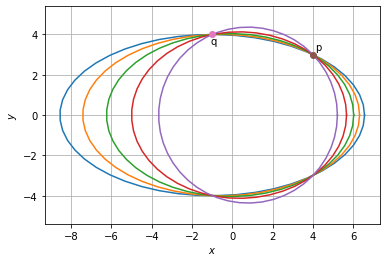
\includegraphics[width=\columnwidth]{solutions/su2021/2/37/figure5_1.png}
\caption{Ellipses passing through the two points with X axis as major axis}
\label{quadforms/37/fig:ellipses}	
\end{figure}
%
